\documentclass[11pt]{article}
\usepackage{amssymb, amsmath, libertine, hyperref, xcolor, booktabs, enumitem, microtype}
\usepackage[T1]{fontenc}
\usepackage[margin=1in]{geometry}
\usepackage{tikz}
\definecolor{dark-red}{rgb}{0.4,0.15,0.15}
\hypersetup{colorlinks, linkcolor=dark-red, citecolor=dark-red, urlcolor=dark-red}
\setlist[enumerate,1]{label=\textbf{\arabic*.}, leftmargin=*, itemsep=10pt}
\setlist[enumerate,2]{label=(\alph*), leftmargin=*, itemsep=4pt, topsep=4pt}
\pagestyle{empty}

\newcommand{\prob}[1]{\medskip\noindent\textbf{\large #1}\par\smallskip}

\begin{document}

\begin{center}
{\Large\bfseries Math 111: Calculus \quad Homework 1}\\[4pt]
{Due Friday, September 18 by 10:00\textsc{p.m.} via Gradescope}
\end{center}

\medskip
\noindent\textbf{Covers} Active Calculus \S1.1 and \S1.3--\S1.5.

\smallskip
\noindent\textbf{Before you start.} Write in sentences and paragraphs, as an
explanation another student in this course could read and follow. Draw diagrams large
and label them. You are encouraged to work with classmates; cite everyone you worked
with, and write your solutions independently --- duplicated solutions are an Honor
Principle violation. Each problem is marked holistically on the 0--5 scale, with up
to two further points for the quality of the writing. If you need an extension, use
the \href{https://docs.google.com/forms/d/e/1FAIpQLSfIfgx44SFtUzefTNr-80yz35MVJaUqQttt96xVTU5mCQCOgg/viewform}{extension
form} \emph{before} the deadline.

\bigskip\hrule\bigskip

%%%%%%%%%%%%%%%%%%%%%%%%%%%%%%%%%%%%%%%%%%%%%%%%%%%%%%%%%%%%%%%%%%%%%%%%%%%%%%%%
\prob{1. A cup of coffee, and how well you can know its rate}

A cup of coffee is left on a desk. Its temperature $T$, in degrees Fahrenheit, is
recorded every two minutes:

\smallskip
\begin{center}
\begin{tabular}{@{}lrrrrrr@{}}
\toprule
$t$ (minutes) & 0 & 2 & 4 & 6 & 8 & 10\\
$T(t)$ ($^\circ$F) & 200 & 185 & 173 & 163 & 155 & 149\\
\bottomrule
\end{tabular}
\end{center}
\smallskip

There is no formula for $T$. The table is all you have.

\begin{enumerate}[resume]
\item[]
\begin{enumerate}
\item Using the table, produce one estimate of $T'(4)$ that you believe is too large
and one that you believe is too small. Give units, and say which is which
\emph{and how you know}.

\item State your best estimate of $T'(4)$, together with a bound on how far off it
could be. Your bound must be one you can defend from the data --- say exactly what you
are assuming about how $T'$ behaves between $t=2$ and $t=6$ in order to defend it.

\item What additional measurement would let you cut your bound roughly in half?
Be specific about when it would be taken.

\item From the table alone, is $T'$ increasing or decreasing over these ten minutes?
Say what your answer means for someone waiting to drink the coffee.
\end{enumerate}
\end{enumerate}

%%%%%%%%%%%%%%%%%%%%%%%%%%%%%%%%%%%%%%%%%%%%%%%%%%%%%%%%%%%%%%%%%%%%%%%%%%%%%%%%
\prob{2. Bicycles and degrees}

Let $B(h)$ be the number of bicycles that cross the Hawthorne Bridge on a day whose
high temperature is $h$ degrees Fahrenheit. Suppose $B(60) = 4300$ and $B'(60) = 210$.

\begin{enumerate}[resume]
\item[]
\begin{enumerate}
\item Explain, in one or two sentences a reader who has never taken calculus could
follow, what $B'(60) = 210$ says about bicycles and weather. State the units of
$B'(60)$ and say where they come from.

\item Would you expect $B'(95)$ to be positive or negative? Explain your reasoning
in terms of the situation, not in terms of formulas.

\item A classmate writes: ``$B'(60) = 210$ means that $210$ more bicycles cross on a
$61$-degree day than on a $60$-degree day.'' This is not quite right. Explain what is
wrong with it, write down a corrected version, and say under what circumstances the
classmate's sentence would be a good approximation.

\item Suppose you also learn that $B'$ is decreasing for temperatures near $60$
degrees. What does that tell you about bicycle traffic near $60$ degrees? Answer in a
sentence about bridges and weather.
\end{enumerate}
\end{enumerate}

%%%%%%%%%%%%%%%%%%%%%%%%%%%%%%%%%%%%%%%%%%%%%%%%%%%%%%%%%%%%%%%%%%%%%%%%%%%%%%%%
\newpage
\prob{3. Reading a derivative off a picture}

The graph of a function $f$ on $[0,8]$ is shown below. No formula for $f$ is given,
and none is needed.

\smallskip
\begin{center}
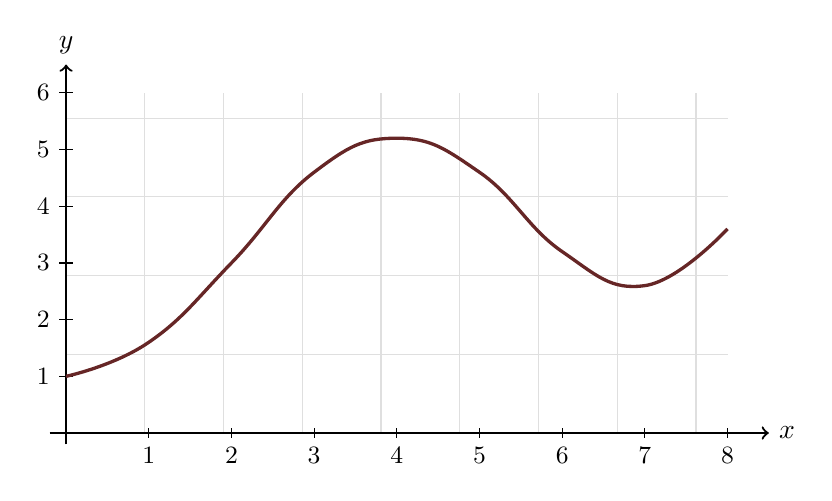
\begin{tikzpicture}[x=1.05cm,y=0.72cm]
  \draw[gray!25] (0,0) grid (8,6);
  \draw[->,thick] (-0.2,0) -- (8.5,0) node[right] {$x$};
  \draw[->,thick] (0,-0.2) -- (0,6.5) node[above] {$y$};
  \foreach \x in {1,...,8} \draw (\x,0.08) -- (\x,-0.08) node[below,font=\small] {\x};
  \foreach \y in {1,...,6} \draw (0.08,\y) -- (-0.08,\y) node[left,font=\small] {\y};
  \draw[very thick, dark-red, smooth, tension=0.75]
    plot coordinates {(0,1) (1,1.6) (2,3) (3,4.6) (4,5.2) (5,4.6) (6,3.2) (7,2.6) (8,3.6)};
\end{tikzpicture}
\end{center}

\begin{enumerate}[resume]
\item[]
\begin{enumerate}
\item On axes of your own, sketch the graph of $f'$ on $[0,8]$. Label the scale on
your vertical axis, and make clear where $f'$ is zero, positive, and negative.

\item Put $f'(1)$, $f'(4)$, and $f'(6)$ in increasing order. Justify the ordering
from the picture of $f$, without reading values off your sketch of $f'$.

\item On which subintervals of $[0,8]$ is $f'$ increasing? Justify your answer using
the shape of the graph of $f$ itself, not by reading your sketch from part (a).

\item Which of the following can you determine from this picture, and which can you
not: $f(3)$, $f'(3)$, and the value of $x$ at which $f'$ is largest? For each, either
give a value or a range you can defend, or explain what makes it undeterminable.
\end{enumerate}
\end{enumerate}

%%%%%%%%%%%%%%%%%%%%%%%%%%%%%%%%%%%%%%%%%%%%%%%%%%%%%%%%%%%%%%%%%%%%%%%%%%%%%%%%
\prob{4. Making examples, and finding the broken step}

\begin{enumerate}[resume]
\item[]
\begin{enumerate}
\item Sketch the graph of a single function $g$ on $[0,4]$ satisfying all of the
following at once: $g(1) = 3$; $g'(1) = 0$; $g'(x) > 0$ for $0 < x < 1$;
$g'(x) < 0$ for $1 < x < 3$; and $g'$ is increasing for $2 < x < 4$. Label the
features that show each condition is met.

\item Give a function $h$ with $h'(2) = 0$ whose graph has neither a peak nor a
valley at $x = 2$. A formula or a carefully drawn graph is fine. Explain how you know
your example works.

\item A student submits the following argument.

\smallskip
\begin{quote}
\textbf{Claim.} If $f$ is increasing on an interval, then $f'$ is increasing on that
interval.

\textbf{Argument.} Suppose $f$ is increasing. Then $f(b) > f(a)$ whenever $b > a$ in
the interval. So the difference quotient $\dfrac{f(b)-f(a)}{b-a}$ is positive for every
such pair. Taking $b$ close to $a$, it follows that $f'(a)$ is positive at every point
of the interval. A positive quantity gets larger as $x$ increases, so $f'$ is increasing.
\end{quote}
\smallskip

Identify the \emph{first} sentence of the argument that is wrong, and say precisely
what is wrong with it. Then give a specific function showing the claim itself is
false. Finally, state a correct claim of the same shape --- something true that the
first part of this argument does establish --- and say why it is true.
\end{enumerate}
\end{enumerate}

\end{document}
